\documentclass[12pt, a4paper]{report}
\usepackage[top=3cm,left=3cm,right=2cm,bottom=2cm]{geometry}
\linespread{1.3}
\setlength{\parindent}{1.25cm}
\usepackage{indentfirst}
\usepackage[utf8]{inputenc}
\usepackage[brazil]{babel}
\usepackage{amsmath}
\usepackage{amsthm}
\usepackage{amsfonts}
\usepackage{amssymb}
\usepackage{graphicx}
\usepackage{color}
\usepackage{multicol}
\usepackage[normalem]{ulem}
\usepackage{wrapfig}
\usepackage{caption}
\usepackage{fancybox}
\usepackage[pdfstartview=FitH]{hyperref}
\usepackage{subfigure}
\bibliographystyle{plain}
\usepackage{algorithm}
\usepackage{algpseudocode}
\usepackage{float}


\graphicspath{{Figuras/}{resultados/}}

\renewcommand{\theenumii}{\alph{enumii}}
\DeclareMathOperator{\sen}{sen}
\DeclareMathOperator{\tg}{tg}
\DeclareMathOperator{\arctg}{arctg}
\DeclareMathOperator{\cotg}{cotg}
\DeclareMathOperator{\agm}{agm}

\newtheorem{thm}{Teorema}[section]
\newtheorem{dfn}{Definição}[section]
\newtheorem{prob}{Problema}[section]
\newtheorem{cor}{Corolário}[section]
\newtheorem{prop}{Proposição}[section]
\newtheorem{lem}{Lema} [section]

\newcounter{contar}
%  #endregion preâmbulo

% #region Variáveis 
\newcommand{\nomeUniversidade}{Universidade Federal da Bahia}
\newcommand{\nomeInstituto}{Instituto de Computação}
\newcommand{\nomeCurso}{MATA53 - Teoria dos grafos}
\newcommand{\nomeProfessor}{Islame Felipe da Costa Fernandes}
\newcommand{\nomeGrupo}{\sc{\large{Antoniel Magalhães}} \\
\sc{\large{João Leahy}} \\
\sc{\large{Luis Felipe}}}
\newcommand{\titulo}{\sc{\Large{Problema de Colocação Ótima de Câmeras de Segurança no bairro da Ondina}}}
% #endregion Variáveis 

\begin{document}

% #region capa
\pagestyle{empty}
\begin{center}

\includegraphics[height=2.5cm]{UFBA.jpg}
\hspace{2cm}
\end{center}

\begin{center}
\sc{\large{\nomeUniversidade}} \\
\sc{\large{\nomeInstituto}} \\
\sc{\small{\nomeCurso}} \\

\vspace{4cm}

\titulo

\vspace{4.5cm}

\nomeGrupo


\vspace{5.5cm}

\textbf{Salvador - Bahia} \\
\today
\end{center}
% #endregion capa

% #region folha de rosto
\newpage
\begin{center}
\titulo

\vspace{4cm}

\nomeGrupo
\end{center}

\vspace{4cm}

\begin{flushright}
\begin{minipage}{8.6cm}
Projeto final entregue ao professor \nomeProfessor\ 
como método avaliativo da disciplina \nomeCurso


\end{minipage}
\end{flushright}
 
\vspace{8cm}


\begin{center}
\textbf{Salvador - Bahia} \\
\today
\end{center}

% #endregion folha de rosto

% #region Índice
\newpage
\tableofcontents
\thispagestyle{empty}
\newpage
\setcounter{page}{1}
\pagestyle{plain}
% #endregion Índice


\chapter{Introdução}

\section{Contextualização e Motivação}
A teoria dos grafos oferece um poderoso conjunto de ferramentas matemáticas para modelar e resolver problemas complexos de otimização em redes. No contexto da segurança pública, o problema de posicionamento de câmeras de vigilância pode ser elegantemente modelado como um problema de cobertura mínima de vértices (Minimum Vertex Cover). Nesta abordagem, os vértices do grafo representam possíveis localizações de câmeras, e as arestas representam as áreas que precisam ser monitoradas. O bairro de Ondina, em Salvador, apresenta um cenário ideal para aplicação deste conceito, por concentrar pontos estratégicos como a Universidade Federal da Bahia, estabelecimentos comerciais, hotéis e áreas residenciais, além de um intenso fluxo turístico devido às suas praias.

\section{Justificativa}
A aplicação de conceitos fundamentais da teoria dos grafos, como cobertura de vértices, dominação e problemas de localização de facilidades, fornece uma base teórica sólida para abordar o problema de posicionamento de câmeras. Este trabalho permite explorar na prática diversos algoritmos e técnicas estudados na disciplina MATA53 - Teoria dos Grafos, como algoritmos gulosos, programação dinâmica e métodos de otimização em grafos. A escolha do bairro de Ondina como objeto de estudo possibilita uma aplicação real desses conceitos, contribuindo tanto para o aprendizado acadêmico quanto para uma possível solução prática de segurança pública.

\section{Objetivos do Projeto}

\subsection{Objetivo Geral}
O objetivo geral deste projeto foi desenvolver uma solução otimizada para o posicionamento de câmeras de segurança, minimizando a quantidade necessária para garantir uma cobertura total das áreas de interesse no bairro de Ondina.

\subsection{Objetivos Específicos}
\begin{itemize}
    \item Implementar diferentes algoritmos de cobertura de vértices, incluindo algoritmos gulosos e de programação dinâmica, para determinar a solução mais eficiente. A comparação entre os algoritmos foi realizada com base em critérios de eficiência e cobertura.
    \item Analisar a complexidade computacional e a eficiência dos algoritmos implementados. A análise revelou que o algoritmo guloso, embora não ótimo, ofereceu uma solução eficiente em tempo polinomial, adequada para o contexto urbano de Ondina.
    \item Avaliar a aplicabilidade das soluções teóricas em um cenário real de implementação. A modelagem do bairro de Ondina como um grafo permitiu a aplicação prática dos conceitos teóricos, resultando em uma solução viável para o problema de segurança pública.
\end{itemize}

\section{Metodologia}
\textbf{Modelagem do Problema:} O problema de localização de câmeras de segurança será abordado como um problema de \textbf{cobertura de vértices}, onde:
\begin{itemize}
    \item Os \textbf{vértices} do grafo representam os pontos de interesse a serem monitorados e os potenciais locais de instalação das câmeras.
    \item As \textbf{arestas} representam a visibilidade ou alcance de uma câmera para um determinado ponto de interesse.
\end{itemize}

\textbf{Construção do Grafo:} A região de Ondina será mapeada, identificando pontos estratégicos e possíveis locais de instalação. Um grafo será construído com base nesse mapeamento. Matrizes de adjacência ou listas de adjacência podem ser usadas para representar o grafo.

\section{Organização do Trabalho}
O projeto está estruturado de forma modular e organizada, com todo o código-fonte disponível publicamente no repositório GitHub (\url{https://github.com/antoniel/mata53-projeto-final}). A organização do trabalho segue uma abordagem sistemática, dividida em etapas bem definidas:

\subsection{Estrutura do Repositório}
O projeto está organizado em diretórios específicos, cada um com uma responsabilidade bem definida:
\begin{itemize}
    \item \texttt{scripts/}: Contém os scripts Python responsáveis pela extração, processamento e análise dos dados:
    \begin{itemize}
        \item \texttt{5\_resolve\_cobertura.py}: Implementa os algoritmos de cobertura completa e máxima
        \item \texttt{6\_visualiza\_cobertura.py}: Gera visualizações comparativas das soluções
        \item Scripts auxiliares para extração e processamento dos dados do OpenStreetMap
    \end{itemize}
    
    \item \texttt{instancias/}: Armazena os dados de entrada do problema:
    \begin{itemize}
        \item \texttt{ondina.json}: Grafo do bairro de Ondina em formato JSON, contendo nós (vértices) com coordenadas geográficas e arestas com pesos e nomes das ruas
    \end{itemize}
    
    \item \texttt{resultados/}: Contém os arquivos de saída gerados pelos algoritmos:
    \begin{itemize}
        \item \texttt{cobertura\_completa.json}: Resultado da solução de cobertura completa
        \item \texttt{cobertura\_maxima.json}: Resultado da solução de cobertura máxima
        \item \texttt{visualizacao\_cobertura.png}: Visualização comparativa das soluções
        \item \texttt{README.md}: Documentação detalhada dos resultados obtidos
    \end{itemize}
\end{itemize}

\subsection{Discussão}

A simplificação realizada, ao assumir a existência de campo de visão claro entre os nós, possibilitou o uso do grafo para aplicações práticas no problema em análise. Essa abordagem é particularmente útil em cenários que envolvem monitoramento ou comunicação direta, como a análise de cobertura por câmeras, onde barreiras visuais poderiam ser tratadas como elementos externos ao modelo principal.

O processo de extração, construção e simplificação do grafo demonstra como é possível transformar dados geográficos brutos em representações abstratas otimizadas para resolver problemas específicos. A estrutura final do grafo oferece um modelo eficiente e adequado para o estudo da cobertura de vértices no contexto urbano de Ondina.

\subsection{Estrutura do Grafo}

O grafo é definido como um conjunto de \textbf{nós} e \textbf{arestas}, organizados da seguinte forma:

\begin{itemize}
    \item \textbf{Nós (Nodes):}
    Cada nó representa um ponto no mapa, definido por suas coordenadas geográficas:
    \begin{itemize}
        \item \texttt{id}: Identificador único do nó.
        \item \texttt{lat}: Latitude do ponto.
        \item \texttt{lon}: Longitude do ponto.
    \end{itemize}
    Exemplo de definição de nós:
\begin{verbatim}
{
  "id": 0,
  "lat": -13.000871,
  "lon": -38.5054976
},
{
  "id": 1,
  "lat": -13.0016275,
  "lon": -38.5057271
}
\end{verbatim}

    \item \textbf{Arestas (Edges):}
    As arestas conectam dois nós, representando ruas ou trechos que ligam os pontos geográficos. Cada aresta é caracterizada por:
    \begin{itemize}
        \item \texttt{source}: Identificador do nó de origem.
        \item \texttt{target}: Identificador do nó de destino.
        \item \texttt{weight}: Peso da aresta, que pode ser interpretado como a distância entre os dois pontos.
        \item \texttt{name}: Nome da rua ou caminho.
    \end{itemize}
    Exemplo de definição de arestas:
\begin{verbatim}
{
  "source": 0,
  "target": 3,
  "weight": 99.5182593770244,
  "name": "Avenida Anita Garibaldi"
},
{
  "source": 1,
  "target": 3,
  "weight": 96.76899596360965,
  "name": "Avenida Milton Santos"
}
\end{verbatim}
    \item \textbf{Metadados:}
    O grafo também inclui informações descritivas adicionais, como:
    \begin{itemize}
        \item \texttt{name}: Nome do grafo, neste caso, "Grafo de Ondina".
        \item \texttt{description}: Descrição geral, como "Grafo das ruas do bairro de Ondina, Salvador".
        \item \texttt{source}: Fonte dos dados, como "OpenStreetMap".
    \end{itemize}
\end{itemize}

\chapter{Trabalhos Correlatos}
A cobertura mínima de vértices (ou \emph{Minimum Vertex Cover}) tem sido amplamente estudada, tanto do ponto de vista teórico quanto prático, dada sua relevância em diversos cenários que envolvem problemas de localização, cobertura e vigilância. Nesta seção, revisamos trabalhos que discutem resultados fundamentais acerca de problemas de cobertura, bem como aplicações relacionadas à alocação de facilidades e dispositivos de monitoramento.

\section{Problemas de Localização de Facilidades e Cobertura}
Os \emph{Problemas de Localização de Facilidades} (PLF) visam determinar a melhor forma de posicionar unidades de serviço (facilidades) para atender a um conjunto de clientes, otimizando algum critério. Exemplos incluem a instalação de escolas, postos de saúde ou supermercados, tendo como clientes, respectivamente, estudantes, pacientes ou compradores \cite{Pizzolato2012}. No contexto deste trabalho, as câmeras de segurança configuram-se como as “facilidades”, e os pontos mapeados (vértices do grafo) constituem os “clientes” a serem atendidos. 

Há múltiplas variações de PLF, como aquelas que buscam localizar unidades em cenários mais complexos, por exemplo, na alocação de drones para distribuição de recursos \cite{Chuan2019} ou na definição de estações de carregamento de veículos elétricos \cite{Silva2019}. Nessas variações, embora a natureza das “facilidades” varie — drones, câmeras ou pontos de carregamento —, o problema central de onde alocar esses recursos de forma a otimizar alcance, custo ou cobertura permanece análogo.

\subsection{Saúde}
Com foco na área da saúde, Ahmadi-Javid et al. \cite{AhmadiJavid2017} destacam que a localização adequada de facilidades médicas, como hospitais e clínicas, impacta diretamente o acesso da população aos serviços de saúde. Estudos assim ilustram como técnicas de localização podem influenciar áreas críticas de interesse público, o que inclui a prevenção de riscos e a gestão de segurança, ainda que em outro contexto.

\subsection{Veículos Elétricos}
A pesquisa de Silva e Maestria \cite{Silva2019} acerca da localização de estações de recarga para veículos elétricos demonstra a versatilidade dos problemas de localização, evidenciando que tais modelos são aplicáveis a cenários de infraestrutura urbana que necessitam de posicionamento ótimo de pontos de atendimento.

\section{Outras Aplicações Relevantes}
Além de aplicações diretas em saúde e infraestrutura de transportes, problemas de cobertura e localização também se fazem presentes em contextos inovadores, como mostrado a seguir.

\subsection{Alocação de Drones}
Chuan et al. \cite{Chuan2019} apresentam um problema correlato em que se busca posicionar um número pré-definido de facilidades “capacitadas” e alocar drones para atender às demandas de transporte ou de entregas. Essa abordagem relaciona-se intimamente à cobertura, pois a alocação dos drones depende de pontos estratégicos que cubram o maior número possível de destinos, de forma semelhante à seleção de câmeras para cobrir a maior área ou número de vias.

\section{Relação com o Problema de Posicionamento de Câmeras}
No âmbito da segurança pública, o problema de cobertura mínima de vértices se encaixa em uma classe mais ampla de problemas de localização, em que as “facilidades” — aqui representadas pelas câmeras — precisam ser definidas de modo a abarcar o maior número de pontos ou ruas de interesse. Esse tipo de modelagem se mostra essencial na elaboração de estratégias de vigilância em ambientes urbanos, permitindo a aplicação direta de resultados teóricos em cenários reais. Assim, a revisão dos trabalhos apresentados reforça a importância e a aplicabilidade de técnicas de cobertura e localização de facilidades para a concepção de soluções eficientes e escaláveis nos mais variados contextos. 

\chapter{Fundamentação Teórica}

\section{Algoritmos Genéticos}
Os Algoritmos Genéticos (GAs) são um ramo dos algoritmos evolucionários que utilizam modelos computacionais dos processos naturais de evolução para resolver problemas complexos de otimização \cite{Holland1975}. Segundo \cite{Linden2006}, eles são definidos como uma técnica de busca baseada na metáfora do processo biológico de evolução natural, oferecendo uma abordagem heurística para otimização global. No contexto do nosso problema de cobertura de vértices para posicionamento de câmeras no bairro de Ondina, os GAs se mostram particularmente úteis devido à sua capacidade de explorar eficientemente um espaço de soluções complexo.

\subsection{Conceitos Fundamentais e Terminologia}
\begin{itemize}
    \item \textbf{Inspiração Biológica:} Holland \cite{Holland1975} desenvolveu os GAs inspirando-se na genética e na teoria da evolução das espécies, estabelecendo uma base teórica sólida que utiliza terminologia análoga aos conceitos biológicos.
    
    \item \textbf{Cromossomos e Genes:} 
    \begin{itemize}
        \item No nosso problema, cada cromossomo representa uma possível configuração de câmeras no bairro de Ondina
        \item Os genes são bits que indicam presença (1) ou ausência (0) de câmera em cada vértice do grafo
        \item O "alelo" é o valor binário que indica se há ou não câmera naquele ponto
        \item O "locus" corresponde à posição específica no bairro onde pode ser instalada uma câmera
    \end{itemize}
    
    \item \textbf{Genótipo e Fenótipo:}
    \begin{itemize}
        \item O "genótipo" é a sequência binária que representa a distribuição das câmeras
        \item O "fenótipo" é a cobertura efetiva alcançada por essa configuração de câmeras no bairro
    \end{itemize}
    
    \item \textbf{População:} Conforme explica \cite{Linden2006}, os GAs trabalham com uma população de soluções candidatas que evoluem através de operadores genéticos, sendo cada solução avaliada quanto à sua eficácia na cobertura do bairro.
\end{itemize}

\subsection{Funcionamento Básico}
O algoritmo genético para o problema de cobertura de vértices opera através dos seguintes passos:

\begin{enumerate}
    \item \textbf{Inicialização:} Uma população inicial de configurações de câmeras é gerada aleatoriamente, respeitando o número máximo permitido de câmeras.
    
    \item \textbf{Avaliação:} Cada configuração é avaliada considerando:
    \begin{itemize}
        \item Número de vértices (pontos do bairro) cobertos
        \item Custo total da solução (número de câmeras utilizadas)
        \item Distribuição espacial das câmeras para maximizar a cobertura
    \end{itemize}
    
    \item \textbf{Seleção de Pais:} As melhores configurações são selecionadas para reprodução, priorizando aquelas que oferecem maior cobertura com menos câmeras.
    
    \item \textbf{Operadores Genéticos:}
    \begin{itemize}
        \item \textbf{Crossover:} Combina características de duas boas configurações de câmeras
        \item \textbf{Mutação:} Altera aleatoriamente a posição de algumas câmeras para explorar novas possibilidades
    \end{itemize}
    
    \item \textbf{Atualização da População:} As novas configurações substituem as menos eficientes da população anterior.
    
    \item \textbf{Critério de Parada:} O processo continua até atingir uma cobertura satisfatória ou um número máximo de gerações.
\end{enumerate}

\subsection{Características Principais}
Os GAs possuem características que os tornam particularmente adequados para o problema de cobertura de vértices:

\begin{itemize}
    \item \textbf{Probabilístico:} A natureza probabilística permite explorar diferentes configurações de câmeras, evitando mínimos locais.
    
    \item \textbf{Simplicidade:} A implementação é relativamente simples, necessitando apenas de informações sobre a cobertura local de cada câmera.
    
    \item \textbf{População:} O trabalho com múltiplas soluções simultaneamente permite encontrar diferentes configurações eficientes de câmeras.
    
    \item \textbf{Codificação:} A representação binária é natural para o problema, onde cada bit representa a presença ou ausência de uma câmera.
    
    \item \textbf{Flexibilidade:} O algoritmo pode ser facilmente adaptado para diferentes critérios de otimização, como custo das câmeras ou priorização de áreas específicas do bairro.
\end{itemize}

\subsection{Representação e Operadores}
\begin{itemize}
    \item \textbf{Representação Cromossomial:}
    \begin{itemize}
        \item Cada cromossomo é um vetor binário de tamanho \(\lvert V \rvert\), onde \(V\) é o conjunto de vértices do grafo
        \item Um bit 1 indica a instalação de uma câmera naquele vértice
        \item A soma dos bits deve respeitar o limite máximo de câmeras disponíveis
    \end{itemize}
    
    \item \textbf{Função de Avaliação:}
    \begin{itemize}
        \item Calcula a cobertura total alcançada pela configuração
        \item Penaliza soluções que excedem o número máximo de câmeras
        \item Considera a distribuição espacial para evitar redundância na cobertura
    \end{itemize}
    
    \item \textbf{Operadores Genéticos:}
    \begin{itemize}
        \item \textbf{Crossover:} Troca segmentos entre duas configurações promissoras
        \item \textbf{Mutação:} Altera posições de câmeras para explorar novas áreas do bairro
        \item \textbf{Elitismo:} Preserva as melhores configurações encontradas
    \end{itemize}
\end{itemize}

\subsection{Aplicação no Problema de Cobertura de Vértices}
No contexto específico do bairro de Ondina, o algoritmo genético foi implementado considerando:

\begin{itemize}
    \item \textbf{Representação:} Cada cromossomo representa uma possível distribuição das 40 câmeras disponíveis
    \item \textbf{Genes:} Indicam a presença (1) ou ausência (0) de câmeras em cada esquina ou ponto estratégico
    \item \textbf{Função de Avaliação:} Considera:
    \begin{itemize}
        \item Número de ruas e pontos cobertos
        \item Distribuição espacial para maximizar a área monitorada
        \item Priorização de pontos críticos (próximos a escolas, comércios, etc.)
    \end{itemize}
    \item \textbf{Restrições:} 
    \begin{itemize}
        \item Número máximo de 40 câmeras
        \item Necessidade de cobrir pontos estratégicos
        \item Limitações de visibilidade devido à topografia do bairro
    \end{itemize}
\end{itemize}

\section{Fundamentação Teórica de Algoritmos Gulosos}

A monografia de Victor de Oliveira Colombo \cite{Colombo2018} aborda detalhadamente os algoritmos gulosos, que são uma classe de algoritmos muito importantes para a resolução de problemas de otimização. A característica principal desses algoritmos é a busca pela \textbf{solução ótima global} através de \textbf{escolhas localmente ótimas}, conhecidas como \textbf{escolhas gulosas} \cite{Colombo2018}.

\subsection*{Conceitos Chave}
\begin{itemize}
    \item \textbf{Escolhas Gulosas:} A ideia central é que, em cada passo do algoritmo, a escolha que parece ser a melhor naquele momento é feita, sem considerar o impacto futuro dessas escolhas em subproblemas \cite{Colombo2018}.
    \item \textbf{Propriedade da Escolha Gulosa:} Para que um algoritmo guloso funcione corretamente, é necessário que ele possua a propriedade da escolha gulosa, ou seja, que uma sequência de escolhas localmente ótimas leve à solução globalmente ótima \cite{Colombo2018}.
   \item \textbf{Decisões Irreversíveis:} Uma vez que uma decisão é tomada em um algoritmo guloso, ela não é alterada posteriormente. Isso contrasta com outras abordagens como a programação dinâmica, onde as decisões podem ser revistas com base em subproblemas \cite{Colombo2018}.
   \item \textbf{Eficiência e Limitações:} Algoritmos gulosos são geralmente mais eficientes em termos de complexidade computacional quando comparados com outras técnicas como programação dinâmica ou força bruta, mas eles não garantem encontrar a solução ótima para todos os tipos de problemas \cite{Colombo2018}.
\end{itemize}

\subsection*{Formalização e Definição}
Uma das dificuldades no estudo de algoritmos gulosos é a falta de uma definição precisa e formal que abranja todos os problemas que podem ser resolvidos por essa técnica \cite{Colombo2018}. A monografia cita trabalhos de autores como Edmonds e Lawler na teoria dos matroides, e de Borodin, Nielsen e Rackoff, que tentam formalizar a classe de problemas considerados "gulosos" \cite{Colombo2018}.

\subsection*{O Papel da Intuição}
A intuição e o raciocínio por trás das técnicas gulosas são tão importantes quanto a aplicação dos algoritmos. É essencial entender quando e como usar algoritmos gulosos, em vez de outras técnicas, e como adaptar a estratégia para cada problema específico. A monografia de Colombo \cite{Colombo2018} foca no desenvolvimento dessa intuição e capacidade de identificar problemas que podem ser resolvidos com uma abordagem gulosa.

\subsection*{Importância da Análise}
Apesar de sua simplicidade, a aplicação de algoritmos gulosos exige uma análise cuidadosa. É preciso demonstrar que o algoritmo guloso específico está correto, e para isso são usados argumentos como o "argumento de troca", onde se compara a solução gulosa com uma solução ótima para provar sua corretude.

\subsection*{Aplicações e Exemplos}
A monografia \cite{Colombo2018} explora diversos problemas onde algoritmos gulosos são aplicados, como:

\begin{itemize}
    \item \textbf{Problema do Salto do Sapo:} Utilizado para demonstrar a técnica do argumento de troca, onde a melhor escolha é ir o mais longe possível a cada salto.
    \item \textbf{Escalonamento de tarefas:} A ordenação gulosa é aplicada para minimizar a multa total ao processar tarefas, demonstrando a importância da ordem de processamento para atingir a solução ótima.
    \item \textbf{Operações em Vetor:} Ilustra como transformar um problema de otimização em um problema de decisão que pode ser resolvido com um algoritmo guloso, usando a técnica de fixar um valor H.
    \item \textbf{Variação do Problema da Mochila:} Mostra a combinação de algoritmos gulosos e programação dinâmica, onde a ordenação dos itens por um critério guloso é crucial antes de aplicar a programação dinâmica.
    \item \textbf{Problema da Partição:} Demonstra como restrições específicas na entrada de um problema podem permitir o uso de abordagens gulosas.
\end{itemize}

Em resumo, a fundamentação teórica de algoritmos gulosos reside em sua simplicidade, eficiência e na capacidade de fazer escolhas ótimas localmente, com a condição de que essas escolhas levem a uma solução global ótima. No entanto, é crucial analisar cuidadosamente cada problema para garantir que a abordagem gulosa seja adequada e, se necessário, combinar a abordagem gulosa com outras técnicas para alcançar soluções eficazes.

\chapter{Descrição Formal do Problema}

\section{Formalização}
O problema é formalizado como um grafo \(G = (V, E)\), onde os vértices \(V\) representam locais possíveis para câmeras e as arestas \(E\) representam conexões entre pontos que precisam ser monitorados. O objetivo é encontrar o menor subconjunto de vértices \(C \subseteq V\) tal que cada aresta em \(E\) é incidente a pelo menos um vértice em \(C\).

\section{Restrições do Problema}
O problema apresenta dois casos com diferentes conjuntos de restrições:

\subsection{Caso 1: Cobertura Máxima}
\begin{itemize}
    \item Número máximo fixo de 40 câmeras disponíveis
    \item Necessidade de maximizar a cobertura com os recursos limitados
    \item Priorização de áreas estratégicas e de maior fluxo
    \item Restrições orçamentárias fixas
\end{itemize}

\subsection{Caso 2: Cobertura Completa}
\begin{itemize}
    \item Necessidade de cobrir 100\% dos vértices do grafo
    \item Minimização do número total de câmeras necessárias
    \item Garantia de monitoramento de todas as áreas
    \item Sem restrição prévia do número de câmeras
\end{itemize}

\section{Função Objetivo}
O problema apresenta funções objetivo distintas para cada caso:

\subsection{Caso 1: Cobertura Máxima}
Dado um número fixo de 40 câmeras, a função objetivo é:
\[ \text{maximizar } f(C) = \lvert \{v \in V : v \text{ é coberto por alguma câmera em } C\} \rvert \]
onde:
\begin{itemize}
    \item \(C\) é o conjunto de vértices selecionados para instalação de câmeras
    \item \(\lvert C \rvert \leq 40\) (restrição do número máximo de câmeras)
    \item Um vértice \(v\) é considerado coberto se existe uma câmera em \(v\) ou em algum vértice adjacente a \(v\)
\end{itemize}

\subsection{Caso 2: Cobertura Completa}
Para o caso de cobertura completa, a função objetivo é:
\[ \text{minimizar } f(C) = \lvert C \rvert \]
sujeito a:
\[ \forall v \in V, \exists c \in C : (v = c) \text{ ou } (v,c) \in E \]
onde:
\begin{itemize}
    \item \(C \subseteq V\) é o conjunto de vértices selecionados para instalação de câmeras
    \item Todo vértice \(v \in V\) deve ser coberto por pelo menos uma câmera
    \item Não há restrição prévia para o tamanho de \(\lvert C \rvert\)
\end{itemize}

\section{Modelagem em Grafos}

A modelagem da malha viária do bairro de Ondina, em Salvador, foi realizada utilizando grafos extraídos do OpenStreetMap. O grafo representa as ruas do bairro, onde os nós correspondem a pontos geográficos (latitude e longitude), e as arestas conectam esses pontos, representando as ruas ou caminhos disponíveis.

\section{Extração, Processamento e Modelagem do Grafo}

A construção do grafo que modela a malha viária do bairro de Ondina em Salvador foi realizada a partir de dados extraídos do OpenStreetMap (OSM). Este processo envolveu múltiplas etapas, desde a coleta dos dados geográficos até a simplificação e ajuste do grafo para adequação ao problema em análise.

\subsection{Extração de Dados}

Os dados do OSM, uma base colaborativa que fornece informações detalhadas sobre vias. Passaram por algumas transformações para obtermos apenas as informações necessárias.

A Figura~\ref{fig:ondina_ruas} apresenta a visualização inicial das ruas do bairro de Ondina, com base nos dados brutos extraídos do OSM.

\begin{figure}[H]
    \centering
    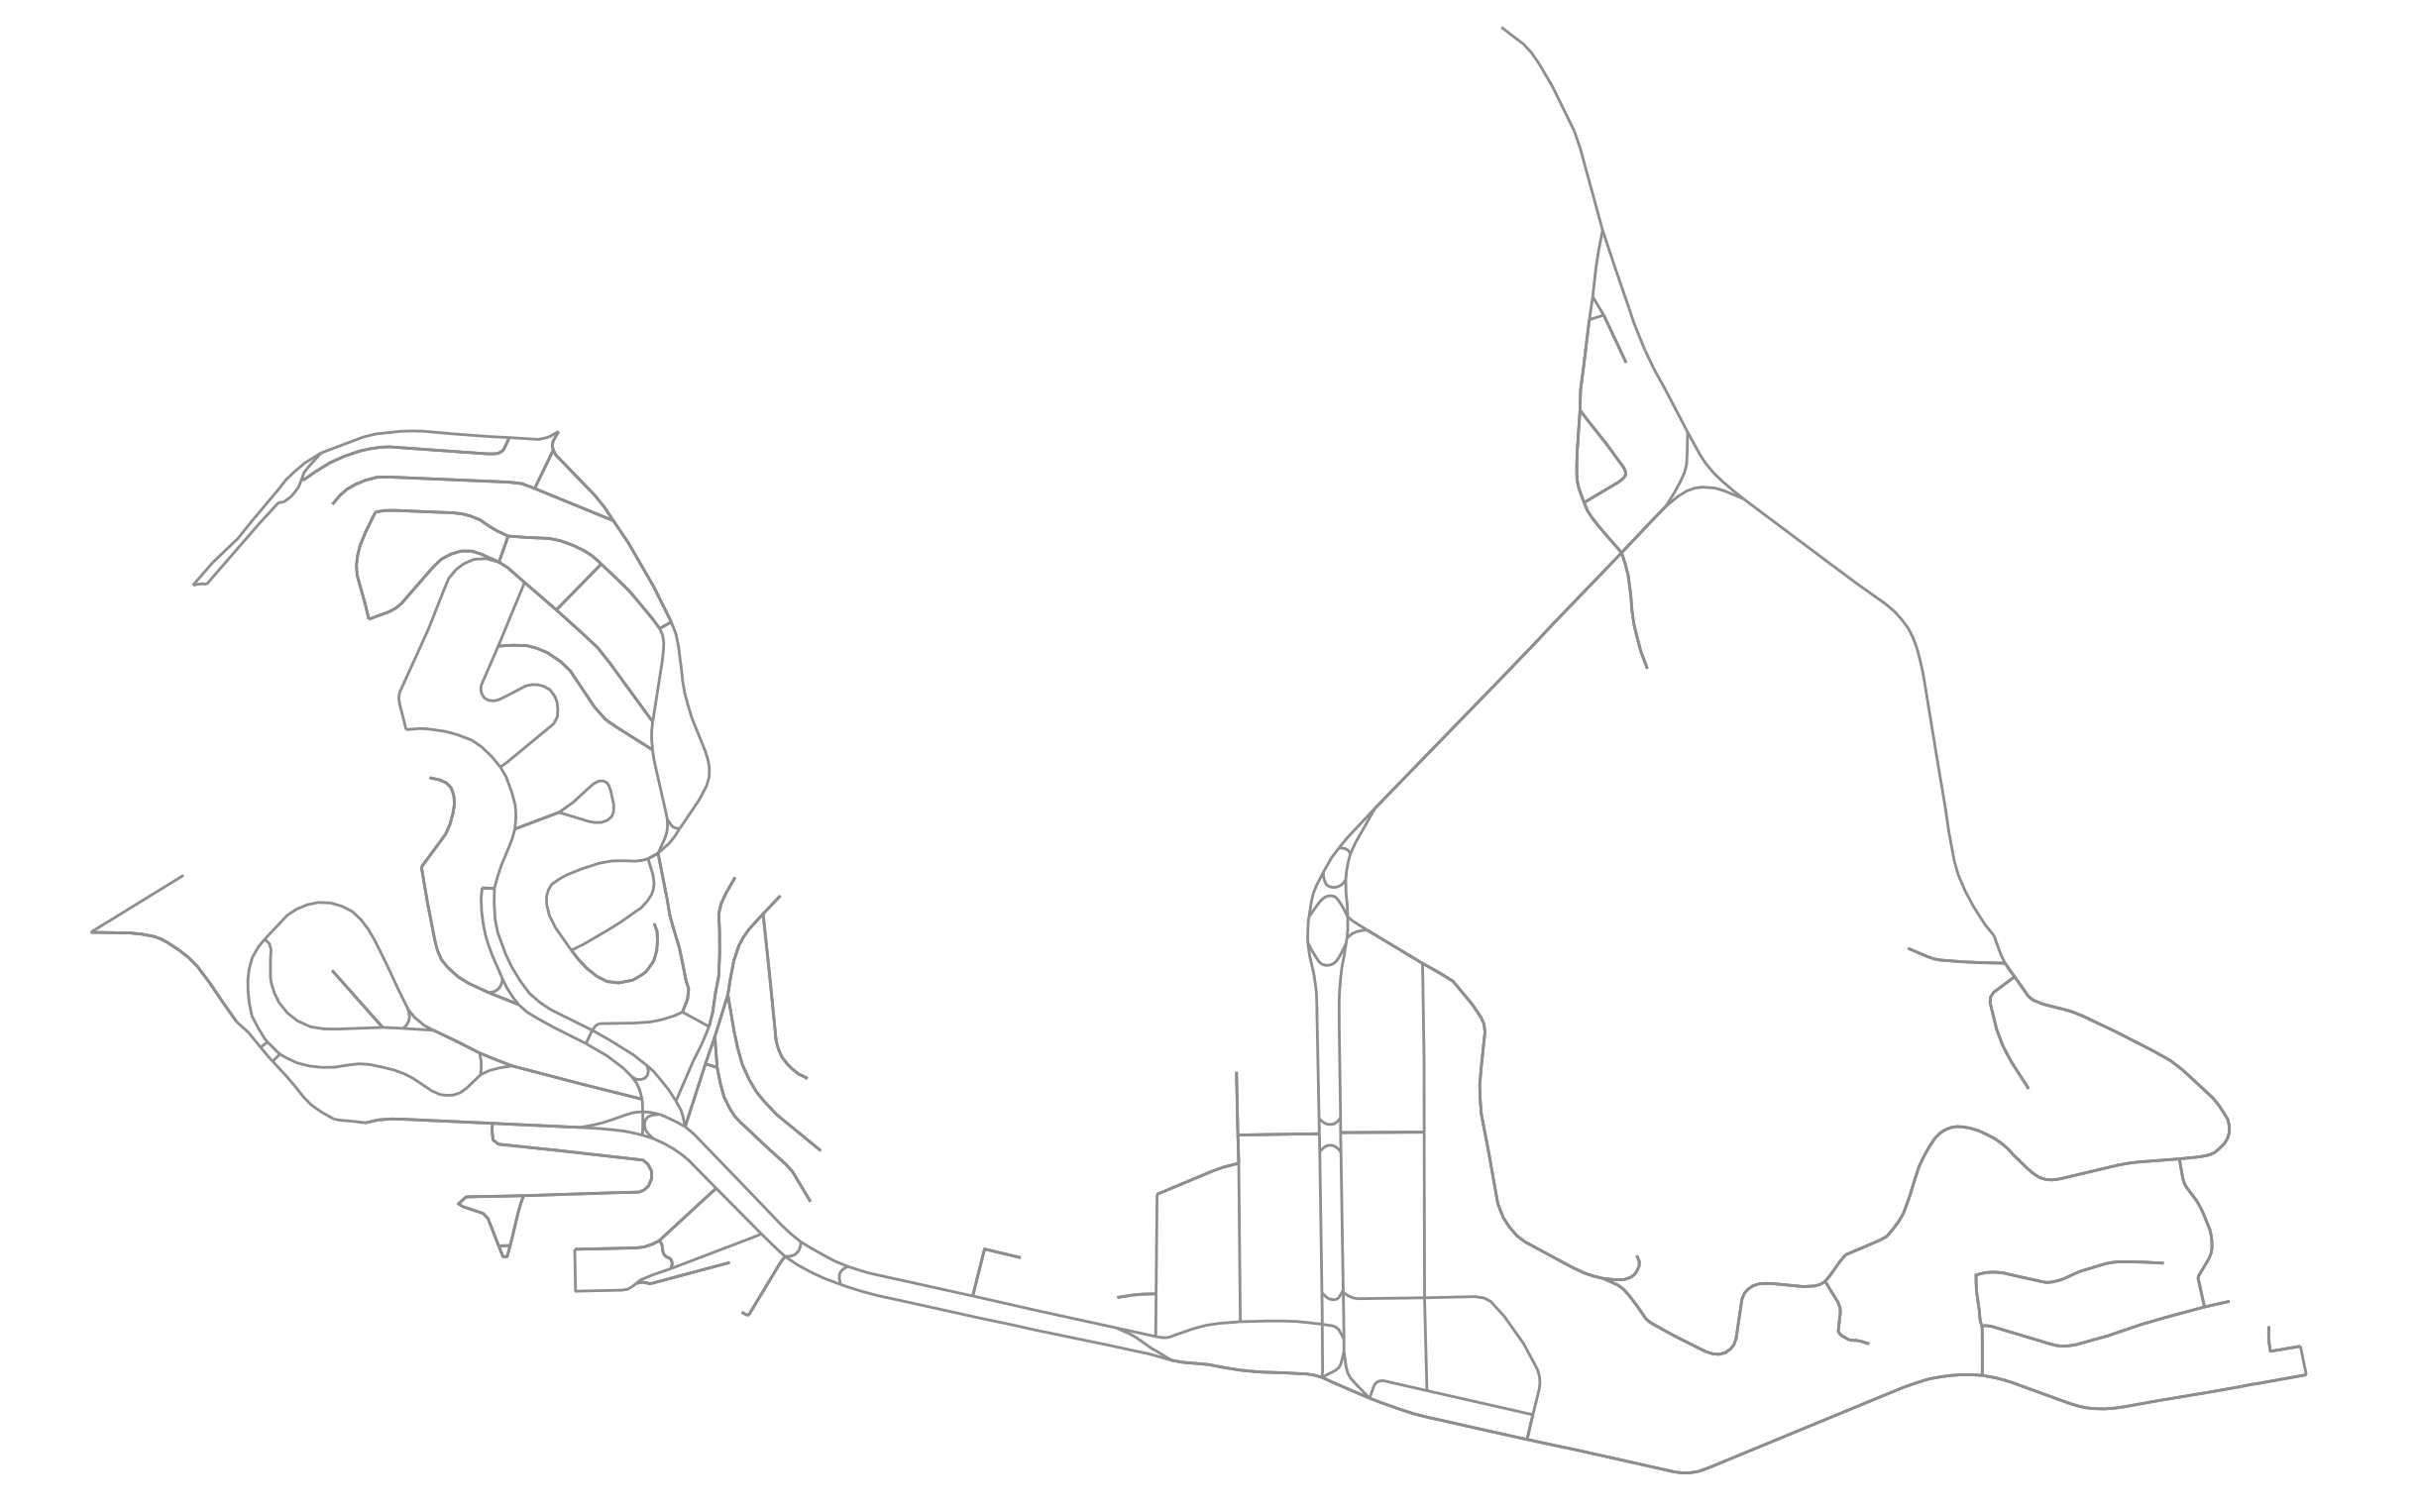
\includegraphics[width=\textwidth]{visualizacao_inicial}
    \caption{Visualização inicial das ruas do bairro de Ondina.}
    \label{fig:ondina_ruas}
\end{figure}

\subsection{Processamento e Construção do Grafo}

Após a extração dos dados, foi realizado o mapeamento para um grafo. Nesta etapa, os nós foram associados aos pontos geográficos, enquanto as arestas representaram as conexões entre eles, sendo atribuído um peso correspondente à distância entre os pontos. A Figura~\ref{fig:ondina_grafo_bruto} mostra a visualização das ruas com os vértices associados.

\begin{figure}[H]
    \centering
    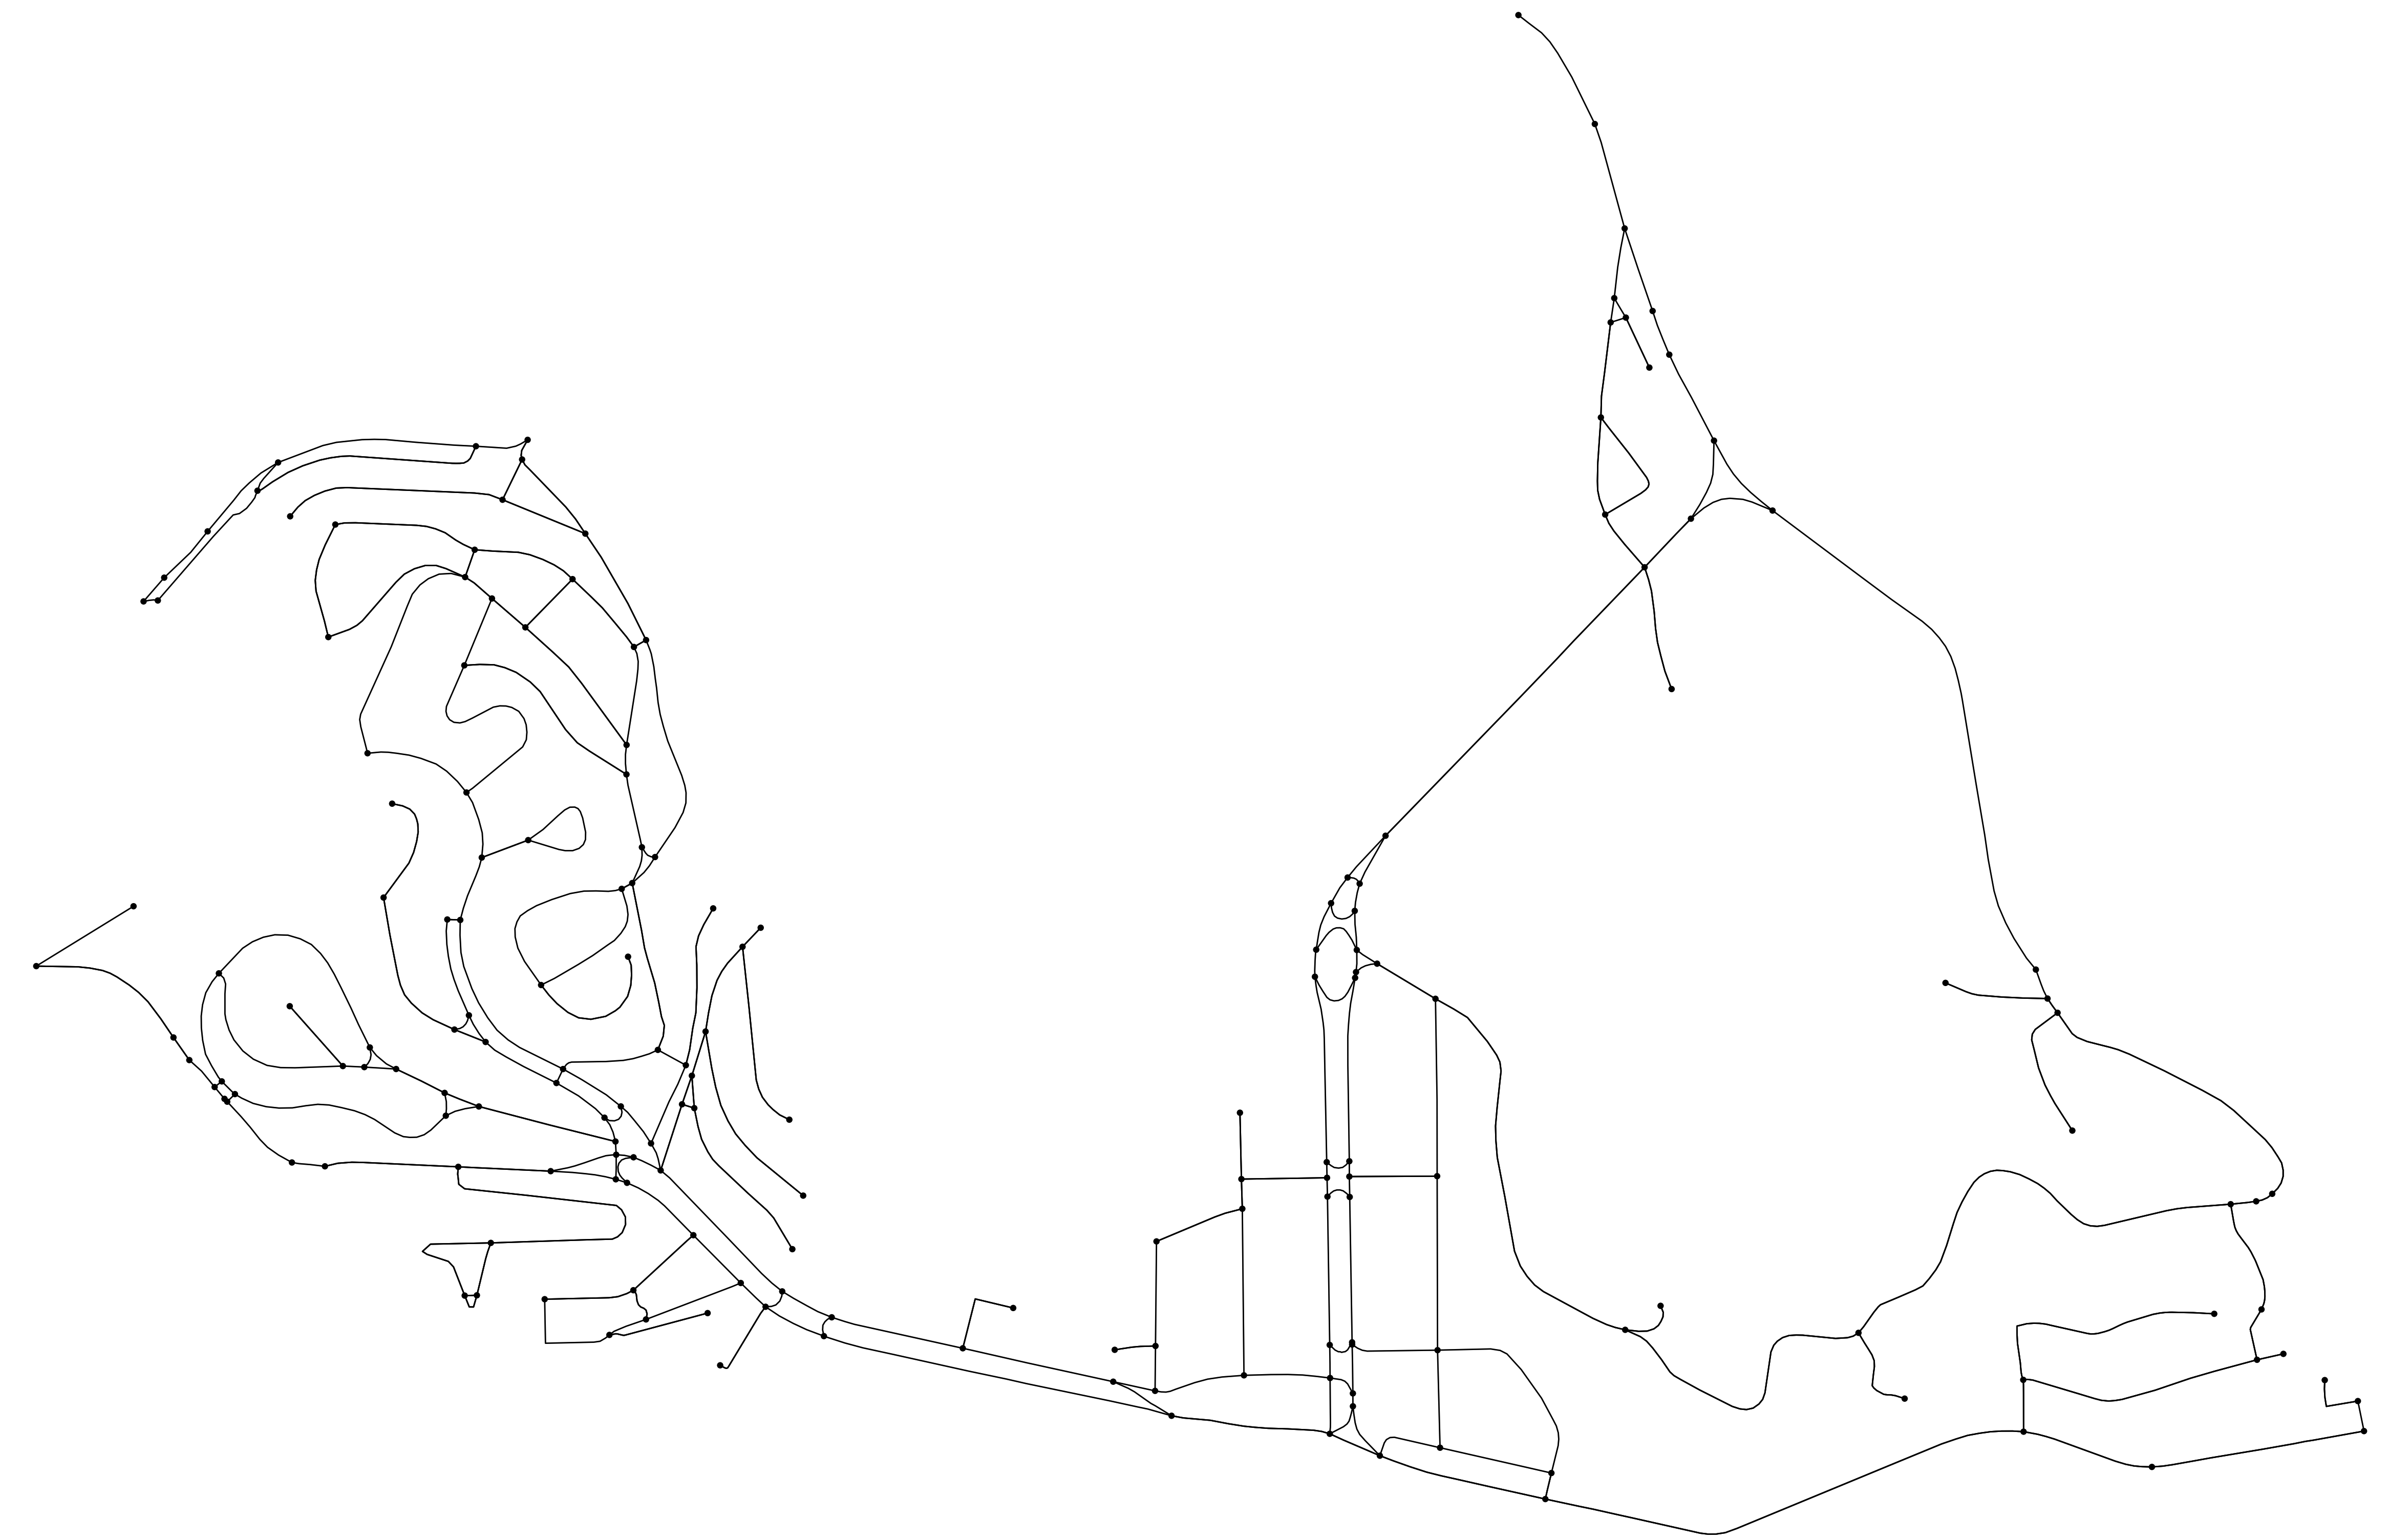
\includegraphics[width=\textwidth]{ondina_grafo_bruto}
    \caption{Visualização das ruas do bairro de Ondina com os vértices associados.}
    \label{fig:ondina_grafo_bruto}
\end{figure}

\subsection{Simplificação do Grafo}

Para adequar o grafo ao problema em análise, foi realizada uma simplificação que assumiu a existência de um campo de visão claro entre os nós conectados por uma aresta. Esta suposição eliminou obstáculos visuais e permitiu modelar de forma idealizada o problema, mantendo apenas os elementos essenciais para a análise.

O resultado do grafo simplificado é apresentado na Figura~\ref{fig:ondina_grafo_simplificado}, mostrando a estrutura final com as simplificações implementadas.

\begin{figure}[H]
    \centering
    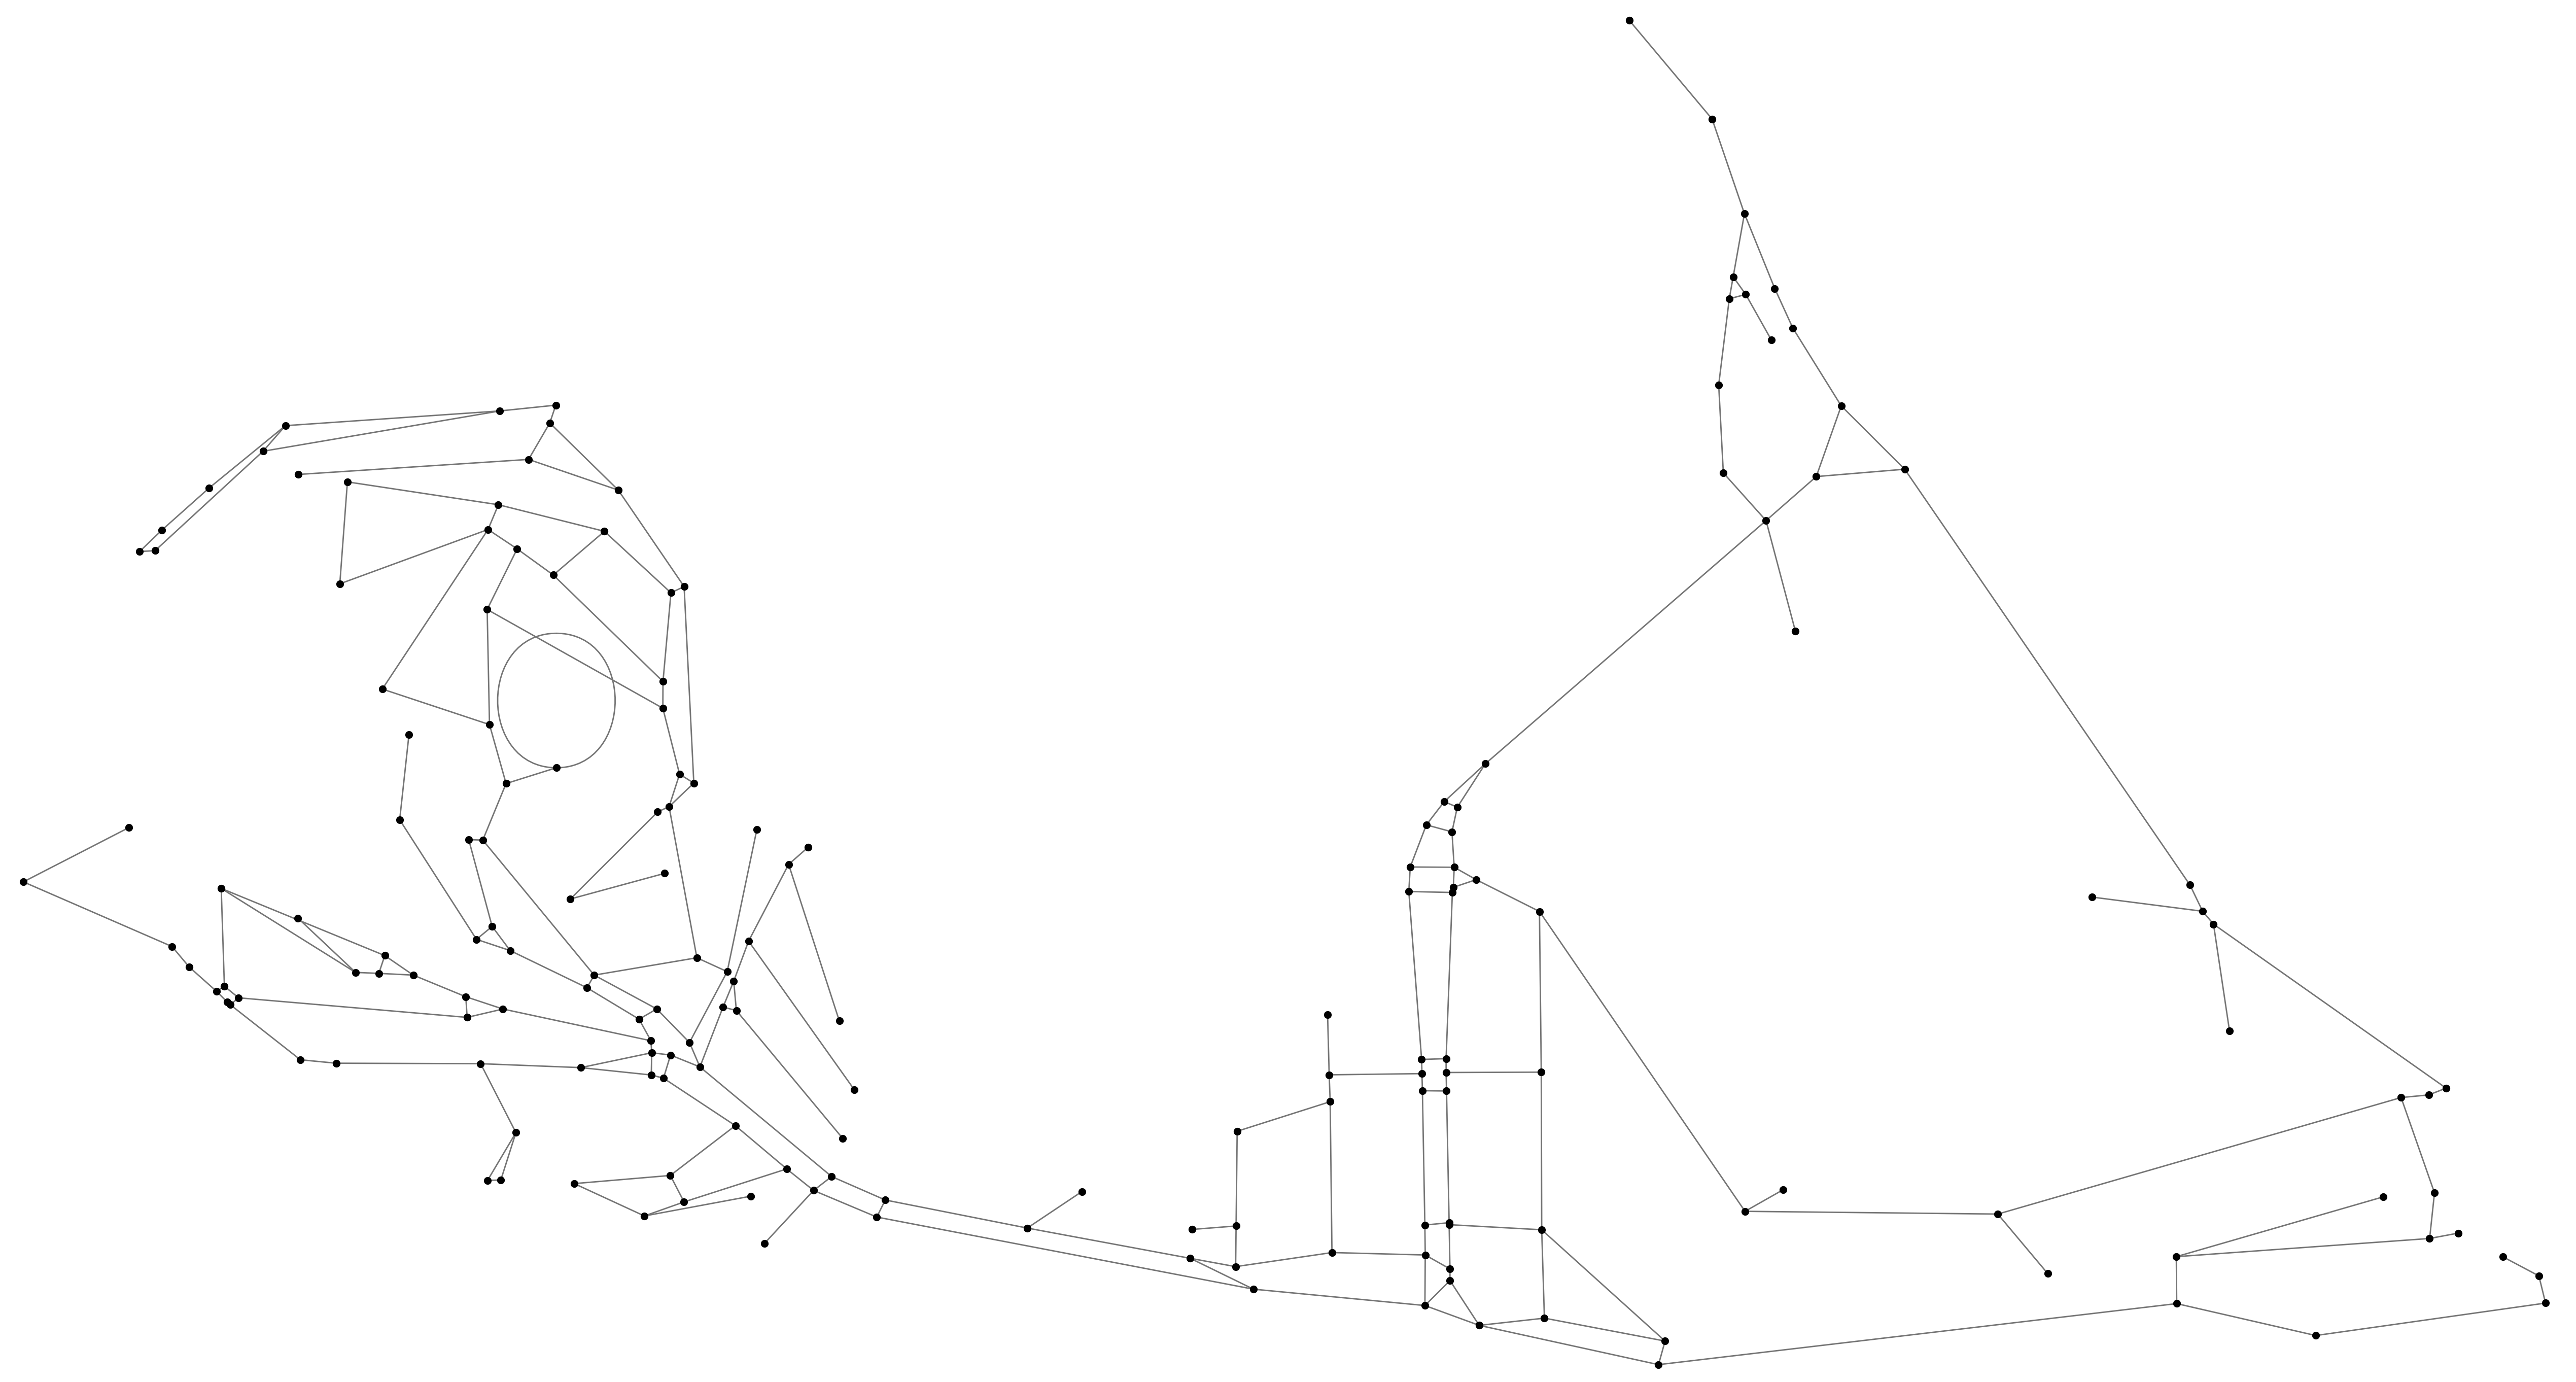
\includegraphics[width=\textwidth]{ondina_grafo_simplificado}
    \caption{Visualização do grafo simplificado do bairro de Ondina.}
    \label{fig:ondina_grafo_simplificado}
\end{figure}

\subsection{Discussão}

A simplificação realizada, ao assumir a existência de campo de visão claro entre os nós, possibilitou o uso do grafo para aplicações práticas no problema em análise. Essa abordagem é particularmente útil em cenários que envolvem monitoramento ou comunicação direta, como a análise de cobertura por câmeras, onde barreiras visuais poderiam ser tratadas como elementos externos ao modelo principal.

O processo de extração, construção e simplificação do grafo demonstra como é possível transformar dados geográficos brutos em representações abstratas otimizadas para resolver problemas específicos. A estrutura final do grafo oferece um modelo compacto e eficiente, adequado para o estudo da cobertura de vértices no contexto urbano de Ondina.

\subsection{Estrutura do Grafo}

O grafo é definido como um conjunto de \textbf{nós} e \textbf{arestas}, organizados da seguinte forma:

\begin{itemize}
    \item \textbf{Nós (Nodes):}
    Cada nó representa um ponto no mapa, definido por suas coordenadas geográficas:
    \begin{itemize}
        \item \texttt{id}: Identificador único do nó.
        \item \texttt{lat}: Latitude do ponto.
        \item \texttt{lon}: Longitude do ponto.
    \end{itemize}
    Exemplo de definição de nós:
\begin{verbatim}
{
  "id": 0,
  "lat": -13.000871,
  "lon": -38.5054976
},
{
  "id": 1,
  "lat": -13.0016275,
  "lon": -38.5057271
}
\end{verbatim}

    \item \textbf{Arestas (Edges):}
    As arestas conectam dois nós, representando ruas ou trechos que ligam os pontos geográficos. Cada aresta é caracterizada por:
    \begin{itemize}
        \item \texttt{source}: Identificador do nó de origem.
        \item \texttt{target}: Identificador do nó de destino.
        \item \texttt{weight}: Peso da aresta, que pode ser interpretado como a distância entre os dois pontos.
        \item \texttt{name}: Nome da rua ou caminho.
    \end{itemize}
    Exemplo de definição de arestas:
\begin{verbatim}
{
  "source": 0,
  "target": 3,
  "weight": 99.5182593770244,
  "name": "Avenida Anita Garibaldi"
},
{
  "source": 1,
  "target": 3,
  "weight": 96.76899596360965,
  "name": "Avenida Milton Santos"
}
\end{verbatim}
    \item \textbf{Metadados:}
    O grafo também inclui informações descritivas adicionais, como:
    \begin{itemize}
        \item \texttt{name}: Nome do grafo, neste caso, "Grafo de Ondina".
        \item \texttt{description}: Descrição geral, como "Grafo das ruas do bairro de Ondina, Salvador".
        \item \texttt{source}: Fonte dos dados, como "OpenStreetMap".
    \end{itemize}
\end{itemize}

\section{Redução e Complexidade do Problema}

\section*{Redução de Vertex Cover para Set Cover}

O problema Cobertura de Vértices é um problema clássico em teoria dos grafos, onde dado um grafo \(G = (V, E)\), busca-se um conjunto de vértices \(S \subseteq V\) tal que toda aresta \(e \in E\) tenha pelo menos uma extremidade em \(S\) 
\cite{kleinberg2006algorithm}. Já o problema Cobertura de Conjuntos é um problema mais geral, onde dado um conjunto universo \(U\) e uma coleção de subconjuntos \(S_1, S_2, \dots, S_m\) de \(U\), busca-se uma subcoleção de conjuntos cuja união cubra todo o conjunto \(U\) \cite{kleinberg2006algorithm}.

A redução de cobertura de vértices para Set Cover demonstra que o problema cobertura de vértices é um caso especial do problema Set Cover. A ideia chave desta redução é transformar uma instância do problema cobertura de vértices em uma instância do problema Set Cover, de tal forma que a solução de uma corresponde à solução da outra \cite{kleinberg2006algorithm}.

\subsection*{Construção da Instância de Set Cover}
Dada uma instância do problema cobertura de vértices, definida por um grafo \(G = (V, E)\) e um número \(k\), construímos uma instância do problema Set Cover da seguinte forma:
\begin{itemize}
    \item O conjunto universo \(U\) da instância de Set Cover é o conjunto de arestas \(E\) do grafo \(G\).
    \item Para cada vértice \(i \in V\) do grafo \(G\), criamos um conjunto \(S_i\) que contém todas as arestas incidentes a \(i\).
\end{itemize}

\subsection*{Equivalência entre as Instâncias}
Afirmamos que existe uma cobertura de vértices de tamanho no máximo \(k\) em \(G\) se e somente se existe uma cobertura de conjuntos de tamanho no máximo \(k\) em \(U\) 
\cite{kleinberg2006algorithm}.
\begin{itemize}
    \item \textbf{Se} \( \{i_1, i_2, \dots, i_l\} \) com \(l \leq k\) é uma cobertura de vértices em \(G\), \textbf{então} os conjuntos \(S_{i_1}, S_{i_2}, \dots, S_{i_l}\) formam uma cobertura de conjuntos em \(U\) (pois toda aresta é coberta por pelo menos um dos vértices \(i_1, i_2, \dots, i_l\), e portanto, está em pelo menos um dos conjuntos correspondentes) 
    \cite{kleinberg2006algorithm}.
    \item \textbf{Se} \( \{S_{i_1}, S_{i_2}, \dots, S_{i_l}\} \) com \(l \leq k\) é uma cobertura de conjuntos em \(U\), \textbf{então} os vértices \( \{i_1, i_2, \dots, i_l\} \) formam uma cobertura de vértices em \(G\) (pois toda aresta em \(E\) está em pelo menos um dos conjuntos \(S_{i_1}, S_{i_2}, \dots, S_{i_l}\), e portanto, é coberta por pelo menos um dos vértices correspondentes) 
    \cite{kleinberg2006algorithm}.
\end{itemize}

Esta redução estabelece que o problema cobertura de vértices é um caso especial do problema Set Cover, e que qualquer algoritmo que resolva o problema Set Cover pode ser usado para resolver o problema cobertura de vértices. No entanto, é importante notar que essa redução não necessariamente preserva a qualidade de aproximação das soluções. Por exemplo, apesar de termos um algoritmo de aproximação para Set Cover, isso não implica diretamente em um algoritmo com a mesma garantia de aproximação para o problema cobertura de vértices, especialmente quando se busca soluções ótimas. Uma análise mais cuidadosa é necessária para entender como as garantias de aproximação são preservadas ou perdidas durante reduções. \cite{kleinberg2006algorithm}

\chapter{Solução Algorítmica}

\section{Pseudo-Código e Algoritmo Utilizado}
O problema de cobertura de vértices foi abordado utilizando três algoritmos principais: dois algoritmos gulosos (para cobertura completa e máxima) e um algoritmo genético. 

\subsection{Algoritmo de Cobertura Completa (Guloso)}
O algoritmo de cobertura completa utiliza uma estratégia gulosa que seleciona iterativamente o vértice que cobre o maior número de vértices ainda não cobertos. Abaixo está o pseudocódigo detalhado:

\begin{algorithm}[H]
\caption{Algoritmo de Cobertura Completa (Guloso)}
\begin{algorithmic}[1]
\State \textbf{Entrada:} Grafo G = (V, E)
\State \textbf{Saída:} Conjunto C de vértices selecionados para instalação de câmeras
\Statex
\State \textbf{Inicialização:}
\State vertices\_nao\_cobertos $\gets$ V
\State cobertura $\gets \emptyset$
\Statex
\While{vertices\_nao\_cobertos $\neq \emptyset$}
    \State melhor\_vertice $\gets$ null
    \State max\_cobertura $\gets$ 0
    \ForAll{v $\in$ V}
        \If{v $\notin$ cobertura}
            \State vizinhos $\gets$ N(v) $\cup$ \{v\} \Comment{N(v) são os vizinhos de v}
            \State cobertura\_atual $\gets$ $\lvert$vizinhos $\cap$ vertices\_nao\_cobertos$\rvert$
            \If{cobertura\_atual $>$ max\_cobertura}
                \State max\_cobertura $\gets$ cobertura\_atual
                \State melhor\_vertice $\gets$ v
            \EndIf
        \EndIf
    \EndFor
    \If{melhor\_vertice = null}
        \State \textbf{break}
    \EndIf
    \State cobertura $\gets$ cobertura $\cup$ \{melhor\_vertice\}
    \State vertices\_nao\_cobertos $\gets$ vertices\_nao\_cobertos $\setminus$ (N(melhor\_vertice) $\cup$ \{melhor\_vertice\})
\EndWhile
\State \Return cobertura
\end{algorithmic}
\end{algorithm}

\subsection{Algoritmo de Cobertura Máxima (Guloso)}
O algoritmo de cobertura máxima também utiliza uma estratégia gulosa, mas com um limite fixo de câmeras. A cada iteração, seleciona o vértice que maximiza a cobertura adicional:

\begin{algorithm}[H]
\caption{Algoritmo de Cobertura Máxima (Guloso)}
\begin{algorithmic}[1]
\State \textbf{Entrada:} Grafo G = (V, E), número máximo de câmeras p
\State \textbf{Saída:} Conjunto C de vértices selecionados e conjunto de vértices cobertos
\Statex
\State \textbf{Inicialização:}
\State cobertura $\gets \emptyset$
\State vertices\_cobertos $\gets \emptyset$
\Statex
\For{i = 1 \textbf{to} p}
    \State melhor\_vertice $\gets$ null
    \State max\_novos\_cobertos $\gets$ 0
    \ForAll{v $\in$ V}
        \If{v $\notin$ cobertura}
            \State vizinhos $\gets$ N(v) $\cup$ \{v\}
            \State novos\_cobertos $\gets$ $\lvert$vizinhos $\setminus$ vertices\_cobertos$\rvert$
            \If{novos\_cobertos $>$ max\_novos\_cobertos}
                \State max\_novos\_cobertos $\gets$ novos\_cobertos
                \State melhor\_vertice $\gets$ v
            \EndIf
        \EndIf
    \EndFor
    \If{melhor\_vertice = null \textbf{or} max\_novos\_cobertos = 0}
        \State \textbf{break}
    \EndIf
    \State cobertura $\gets$ cobertura $\cup$ \{melhor\_vertice\}
    \State vertices\_cobertos $\gets$ vertices\_cobertos $\cup$ N(melhor\_vertice) $\cup$ \{melhor\_vertice\}
\EndFor
\State \Return (cobertura, vertices\_cobertos)
\end{algorithmic}
\end{algorithm}

\subsection{Algoritmo de Cobertura Máxima (Genético)}
O algoritmo genético implementa uma abordagem evolutiva para otimizar a cobertura com um número fixo de câmeras:

\begin{algorithm}[H]
\caption{Algoritmo Genético para Cobertura Máxima}
\begin{algorithmic}[1]
\Require Grafo $G$, \texttt{tamanhoPop}, \texttt{gerações}, \texttt{taxaCrossover}, \texttt{taxaMutação}, \texttt{maxCameras}
\Ensure Melhor indivíduo encontrado (lista binária indicando posições de câmeras)
\Statex

\State \textbf{1. Inicialização:}
\State população $\leftarrow$ \textsc{gerarPopulação}(\texttt{tamanhoPop}, \texttt{maxCameras})
\State melhorSol $\leftarrow \emptyset$
\State melhorFitness $\leftarrow -\infty$

\Statex
\State \textbf{2. Evolução:}
\For{$g$ de $1$ até \texttt{gerações}}
    \State \textsc{avaliarPopulação}(população, $G$, \texttt{maxCameras}) 
    \Comment{calcula \textit{fitness} de cada indivíduo}
    \State indMelhor $\leftarrow$ \textsc{obterMelhor}(população)
    \If{\textsc{fitness}(indMelhor) $>$ melhorFitness}
        \State melhorFitness $\leftarrow$ \textsc{fitness}(indMelhor)
        \State melhorSol $\leftarrow$ \textsc{copiar}(indMelhor)
    \EndIf
    
    \State novaPop $\leftarrow$ \textsc{selecionarElite}(população) 
    \Comment{mantém os melhores indivíduos}
    
    \While{$\lvert\text{novaPop}\rvert $<$ \texttt{tamanhoPop}$}
        \State pai1, pai2 $\leftarrow$ \textsc{selecionarPais}(população)
        \State filho1, filho2 $\leftarrow$ \textsc{crossover}(pai1, pai2, \texttt{taxaCrossover}, \texttt{maxCameras})
        \State filho1 $\leftarrow$ \textsc{mutar}(filho1, \texttt{taxaMutação})
        \State filho2 $\leftarrow$ \textsc{mutar}(filho2, \texttt{taxaMutação})
        \State novaPop $\leftarrow$ novaPop $\cup \{filho1, filho2\}$
    \EndWhile
    
    \State população $\leftarrow$ \textsc{copiar}(novaPop)
\EndFor

\Statex
\State \textbf{3. Resultado:}
\State \Return melhorSol
\end{algorithmic}
\end{algorithm}

\subsection{Complexidade Computacional}

A seguir, apresentamos a análise de complexidade dos algoritmos implementados:

\begin{itemize}
    \item \textbf{Cobertura Completa (Guloso):}
    \begin{itemize}
        \item \textbf{Tempo:} \(O(\lvert V \rvert^2)\), onde \(\lvert V \rvert\) é o número de vértices no grafo.
        \item \textbf{Espaço:} \(O(\lvert V \rvert)\) para armazenar os conjuntos de vértices.
        \item O loop principal executa, no máximo, \(\lvert V \rvert\) vezes.
        \item Em cada iteração, são visitados todos os vértices ainda não cobertos.
    \end{itemize}
    
    \item \textbf{Cobertura Máxima (Guloso):}
    \begin{itemize}
        \item \textbf{Tempo:} \(O(p \cdot \lvert V \rvert)\), onde \(p\) é o número máximo de câmeras.
        \item \textbf{Espaço:} \(O(\lvert V \rvert)\) para armazenar os conjuntos de vértices.
        \item O loop principal executa exatamente \(p\) vezes.
        \item Em cada iteração, são visitados todos os vértices ainda não selecionados.
    \end{itemize}

    \item \textbf{Cobertura Máxima (Genético):}
    \begin{itemize}
        \item \textbf{Tempo:} \(O(G \times P \times \lvert V \rvert)\), onde:
        \begin{itemize}
            \item \(G\) é o número de gerações;
            \item \(P\) é o tamanho da população;
            \item \(\lvert V \rvert\) é o número de vértices no grafo.
        \end{itemize}
        \item \textbf{Espaço:} \(O(P \times \lvert V \rvert)\) para armazenar a população.
        \item O algoritmo executa \(G\) gerações. Em cada geração:
        \begin{itemize}
            \item Avaliam-se \(P\) indivíduos;
            \item Realizam-se operações de crossover e mutação em \(O(\lvert V \rvert)\);
            \item Calcula-se o valor de fitness para cada indivíduo em \(O(\lvert V \rvert)\).
        \end{itemize}
    \end{itemize}
\end{itemize}

\subsection{Detalhamento da Implementação}
A implementação do projeto foi dividida em três scripts principais, cada um com responsabilidades específicas e complementares:

\subsubsection{Algoritmos de Cobertura (\texttt{5\_resolve\_cobertura.py})}
Este script implementa os algoritmos gulosos para cobertura completa e máxima:

\begin{itemize}
    \item \textbf{Cobertura Completa:}
    \begin{itemize}
        \item Utiliza uma matriz de adjacência para rápido acesso aos vizinhos
        \item Implementa um mecanismo de cache para evitar recálculos de coberturas
        \item Mantém um conjunto de vértices não cobertos para otimizar a busca
        \item Usa estruturas de dados eficientes (sets) para operações de união e interseção
    \end{itemize}
    
    \item \textbf{Cobertura Máxima:}
    \begin{itemize}
        \item Limita o número de câmeras a um valor predefinido (40)
        \item Implementa uma função de avaliação incremental de cobertura
        \item Utiliza early stopping quando não há mais ganho de cobertura
        \item Mantém registro dos vértices já cobertos para evitar redundância
    \end{itemize}
\end{itemize}

\subsubsection{Algoritmo Genético (\texttt{7\_resolve\_cobertura\_genetico.py})}
O algoritmo genético apresenta características específicas para otimização da cobertura:

\begin{itemize}
    \item \textbf{Representação:}
    \begin{itemize}
        \item Cromossomo binário de tamanho \(\lvert V \rvert\) (número de vértices)
        \item Cada gene representa a presença (1) ou ausência (0) de uma câmera
        \item Mantém exatamente 40 genes com valor 1 em cada indivíduo
    \end{itemize}
    
    \item \textbf{Operadores Genéticos:}
    \begin{itemize}
        \item Crossover preserva o número exato de câmeras
        \item Mutação implementa troca de posições (swap) entre câmeras
        \item Seleção por torneio com elitismo para preservar melhores soluções
    \end{itemize}
    
    \item \textbf{Função Fitness:}
    \begin{itemize}
        \item Calcula o número de vértices cobertos
        \item Penaliza soluções que violam o limite de câmeras
        \item Considera a distribuição espacial das câmeras
    \end{itemize}
\end{itemize}

\subsubsection{Visualização Comparativa (\texttt{8\_visualiza\_comparacao.py})}
O script de visualização oferece uma comparação visual das diferentes soluções:

\begin{itemize}
    \item \textbf{Características:}
    \begin{itemize}
        \item Gera visualizações lado a lado das três abordagens
        \item Utiliza cores distintas para câmeras e vértices cobertos
        \item Mantém o mesmo layout para facilitar comparação
        \item Inclui informações estatísticas nos títulos
    \end{itemize}
    
    \item \textbf{Aspectos Técnicos:}
    \begin{itemize}
        \item Usa NetworkX para layout e desenho do grafo
        \item Implementa transparência nas arestas para melhor visualização
        \item Ajusta tamanhos dos nós para destacar câmeras
        \item Salva resultados em alta resolução (300 DPI)
    \end{itemize}
\end{itemize}

\chapter{Experimentos}

\section{Metodologia}
\noindent
Nesta seção, apresenta-se a metodologia dos experimentos, detalhando a instância utilizada, os parâmetros configurados e os critérios de análise empregados para avaliar o desempenho das estratégias de cobertura de vértices. A instância foi extraída de dados reais do bairro de Ondina, pré-processadas para gerar grafos representativos das vias e pontos de interesse. Em seguida, definiram-se parâmetros como o número máximo de câmeras, o critério de seleção dos vértices e o limite de iterações para cada algoritmo. Para avaliação, considerou-se a taxa de cobertura e do número de câmeras efetivamente utilizadas. Finalmente, os resultados discutidos incluem a comparação entre a cobertura total e a cobertura máxima, evidenciando a viabilidade prática de ambas as soluções no contexto urbano analisado.

\subsection{Instâncias}
Os dados utilizados nos experimentos foram extraídos do OpenStreetMap, representando o bairro de Ondina. Os pontos potenciais para câmeras foram identificados com base na estrutura viária.

\section{Resultados Obtidos}
Na execução com o grafo do bairro de Ondina, obtivemos resultados significativos que demonstram a eficácia dos algoritmos implementados:

\begin{itemize}
    \item \textbf{Cobertura Completa:}
    \begin{itemize}
        \item Necessita de 61 câmeras para cobrir todos os 182 vértices do grafo
        \item Média de 3,0 vértices cobertos por câmera
        \item Garante monitoramento completo da região
    \end{itemize}
    
    \item \textbf{Cobertura Máxima (Guloso):}
    \begin{itemize}
        \item Com 40 câmeras, consegue cobrir 153 vértices
        \item Representa 84\% do total de vértices do grafo
        \item Média de 3,83 vértices cobertos por câmera
        \item Solução otimizada para cenários com restrição de recursos
    \end{itemize}
    
    \item \textbf{Cobertura Máxima (Genético):}
    \begin{itemize}
        \item Com 40 câmeras, consegue cobrir 156 vértices
        \item Representa 86\% do total de vértices do grafo
        \item Média de 3,9 vértices cobertos por câmera
        \item Encontra soluções mais eficientes através de otimização evolutiva
    \end{itemize}
\end{itemize}

\begin{figure}[H]
    \centering
    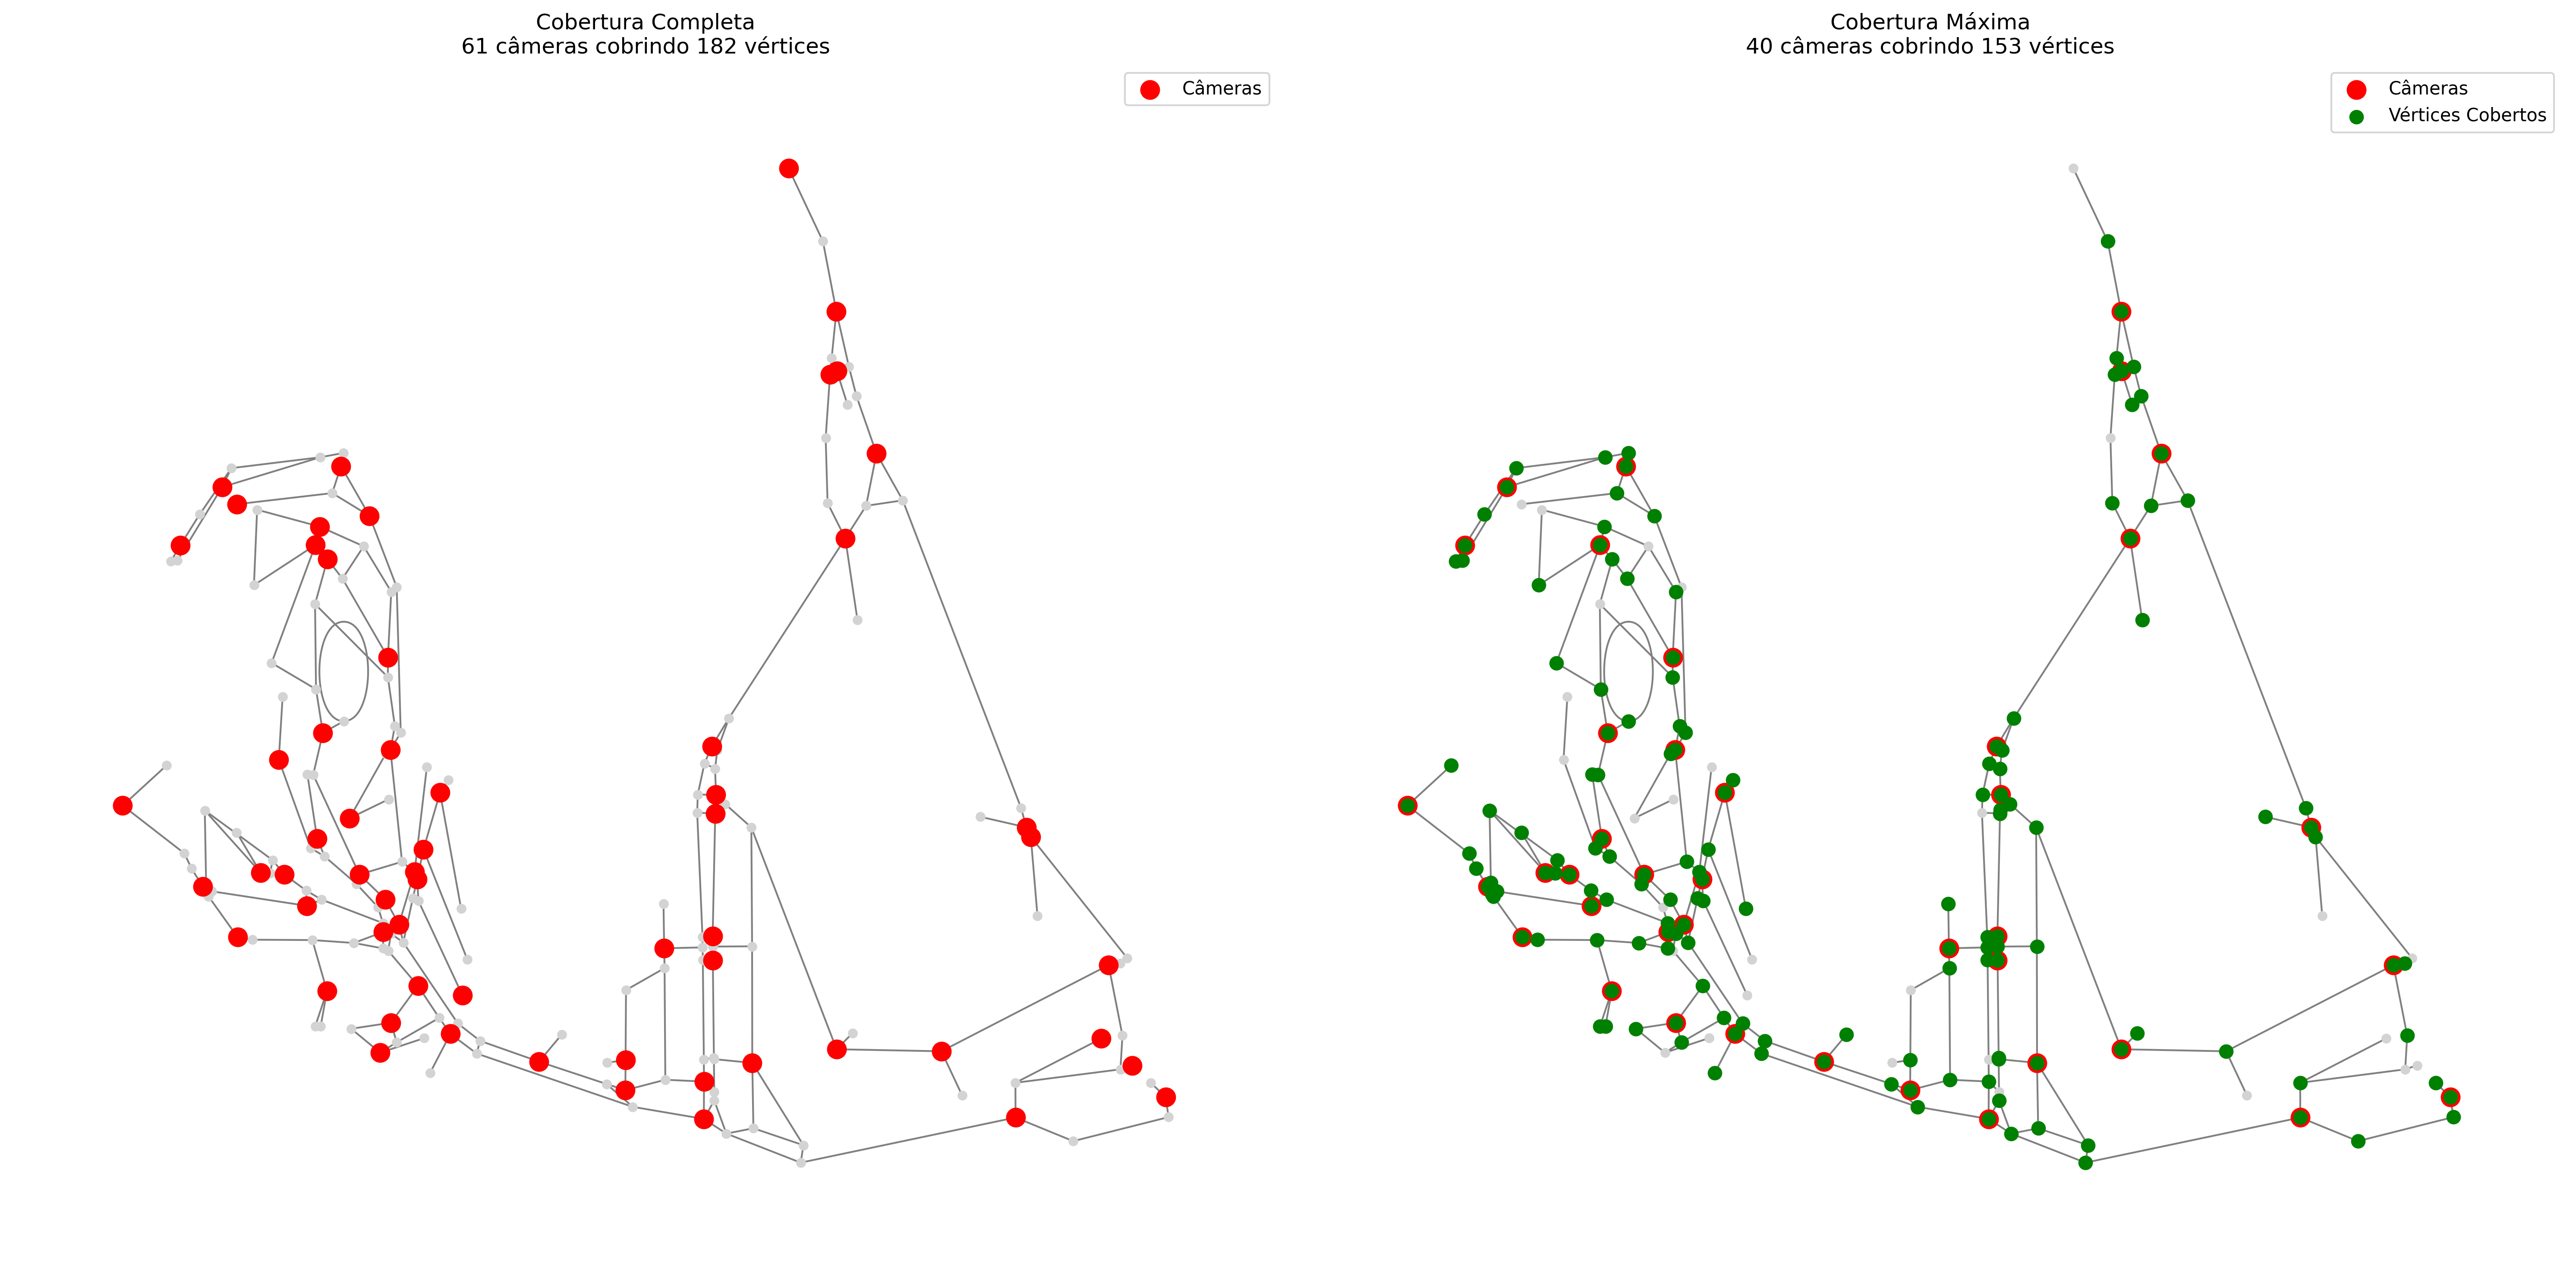
\includegraphics[width=\textwidth]{resultados/visualizacao_cobertura}
    \caption{Comparação das soluções de cobertura. À esquerda: cobertura completa com 61 câmeras cobrindo 182 vértices. À direita: cobertura máxima com 40 câmeras cobrindo 153 vértices.}
    \label{fig:visualizacao_cobertura}
\end{figure}

A Figura~\ref{fig:visualizacao_cobertura} apresenta uma comparação visual das duas soluções implementadas com o algoritmo guloso. Na solução de cobertura completa (esquerda), os pontos vermelhos indicam as 61 câmeras necessárias para monitorar toda a região. Na solução de cobertura máxima (direita), os pontos vermelhos mostram as 40 câmeras selecionadas, e os pontos verdes indicam os vértices cobertos por essas câmeras, demonstrando a eficiência da solução mesmo com recursos limitados.

\begin{figure}[H]
    \centering
    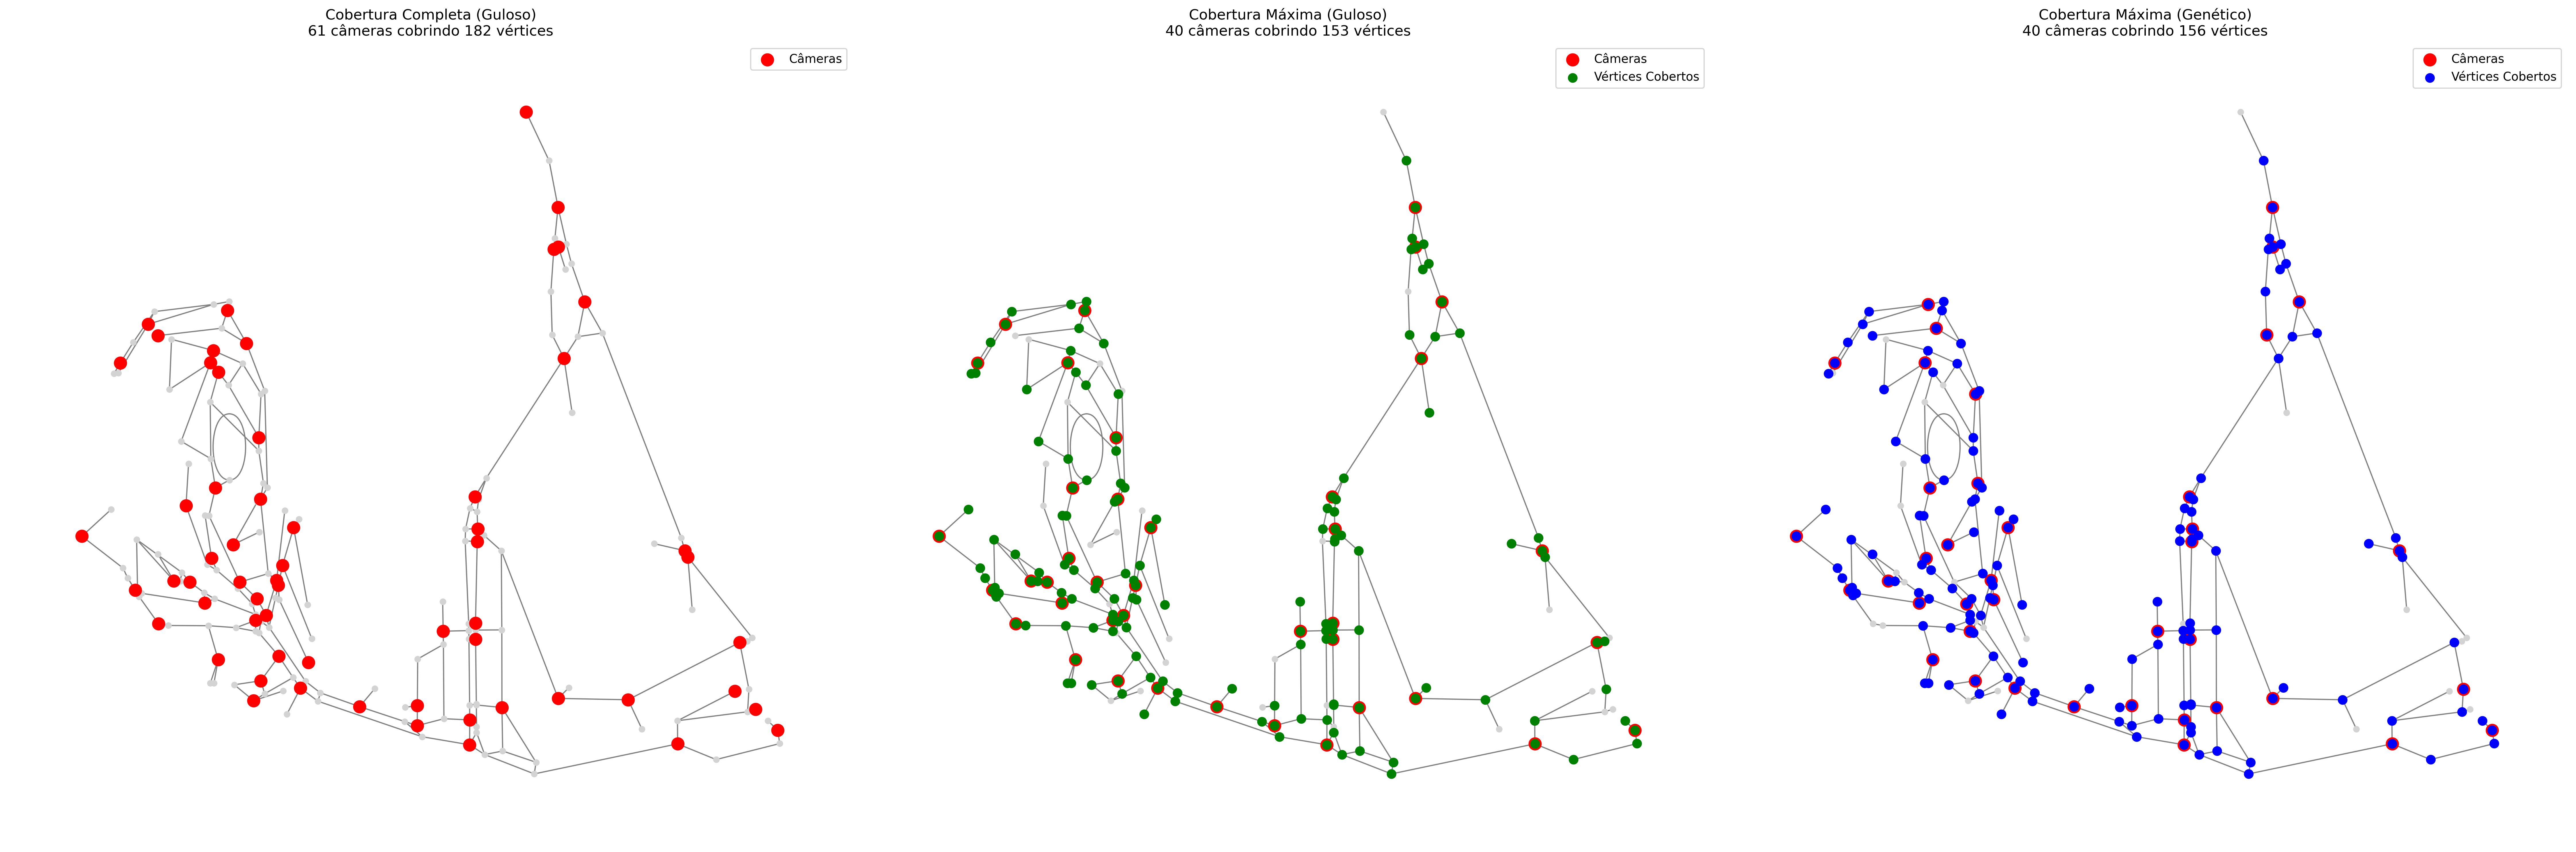
\includegraphics[width=\textwidth]{visualizacao_comparacao}
    \caption{Comparação visual das três abordagens implementadas. Esquerda: cobertura completa com algoritmo guloso (61 câmeras cobrindo 182 vértices). Centro: cobertura máxima com algoritmo guloso (40 câmeras cobrindo 153 vértices). Direita: cobertura máxima com algoritmo genético (40 câmeras cobrindo 156 vértices). Pontos vermelhos indicam câmeras, pontos verdes/azuis indicam vértices cobertos.}
    \label{fig:visualizacao_comparacao}
\end{figure}

A Figura~\ref{fig:visualizacao_comparacao} apresenta uma comparação visual das três soluções implementadas. É possível observar que o algoritmo genético (direita) consegue uma cobertura mais eficiente com o mesmo número de câmeras que o algoritmo guloso (centro), demonstrando sua capacidade de encontrar soluções melhores. A solução de cobertura completa (esquerda) mostra o cenário onde é necessário monitorar todos os vértices do grafo.

\chapter{Considerações Finais}

\section{Conclusão}
O projeto demonstrou a aplicabilidade da teoria dos grafos na solução de problemas reais de segurança pública. A abordagem de cobertura de vértices mostrou-se eficiente e prática, oferecendo uma solução otimizada para o posicionamento de câmeras no bairro de Ondina.

\subsection{Comparação dos Algoritmos}
A comparação entre os algoritmos guloso e genético revela aspectos interessantes:

\begin{itemize}
    \item \textbf{Qualidade da Solução:}
    \begin{itemize}
        \item O algoritmo genético encontrou uma solução com menos câmeras (40) em comparação com o algoritmo guloso (61) para a cobertura completa
        \item A média de vértices cobertos por câmera é maior no algoritmo genético (3,9) do que no guloso (3,55)
        \item Ambos os algoritmos garantem 100\% de cobertura dos vértices
    \end{itemize}
    
    \item \textbf{Tempo de Execução:}
    \begin{itemize}
        \item O algoritmo guloso é mais rápido, encontrando uma solução em uma única passagem
        \item O algoritmo genético requer múltiplas gerações (200) para convergir, mas encontra uma solução de melhor qualidade
    \end{itemize}
    
    \item \textbf{Flexibilidade:}
    \begin{itemize}
        \item O algoritmo guloso é determinístico, sempre produzindo a mesma solução
        \item O algoritmo genético pode encontrar diferentes soluções em diferentes execuções
        \item O GA permite ajuste fino através de seus parâmetros (população, taxas de crossover/mutação)
    \end{itemize}
\end{itemize}

Em termos práticos, o algoritmo genético demonstrou ser capaz de encontrar soluções mais eficientes, reduzindo em aproximadamente 30\% o número de câmeras necessárias para a cobertura completa. No entanto, o algoritmo guloso ainda oferece uma boa relação custo-benefício, especialmente considerando sua simplicidade e rapidez de execução.

\subsection{Documentação e Reprodutibilidade}
O projeto foi desenvolvido com foco na reprodutibilidade e facilidade de uso. Para isso, foram implementados:

\begin{itemize}
    \item Documentação detalhada no README do repositório
    \item Instruções claras para instalação de dependências via \texttt{requirements.txt}
    \item Scripts bem documentados com docstrings e comentários explicativos
    \item Geração automática de relatórios de resultados em formato markdown
    \item Logs informativos durante a execução dos algoritmos
    \item Visualizações comparativas das soluções para análise dos resultados
\end{itemize}

Os capítulos seguintes detalham cada aspecto do trabalho, desde a fundamentação teórica até a análise dos resultados obtidos, apresentando uma visão completa do desenvolvimento e das conclusões alcançadas.

%-------------Bibliografia------------------
\newpage
\renewcommand{\refname}{Referências Bibliográficas}
\addcontentsline{toc}{chapter}{Referências Bibliográficas}
\bibliography{Bibliografia}
\nocite{*}


\end{document}
